% Provenance (never printed): see sources/outline_sources.md (Year 3:
% sequence stratigraphy, accommodation and supply, systems tracts,
% cyclostratigraphy). Brief: sources/book5/BRIEFS.md, ch. 16. Curves from
% figdata/bachelor-3/shelf_model.py and lr04_periodogram.py. Exercise and
% problem values in the Book 5 scratch calculator calc/ch16.py. The Varden
% basin, its shelf and its core are invented.
\chapter{层序地层学}\label{ch:b3:sequence-stratigraphy}

在大陆边缘的地震剖面上，反射层依次超覆于较老的反射层之上，
随后向盆地方向推进，再向陆地方向后退，
这一模式在更高层位重复出现。每一套地层都记录了两种速率之间的较量：
一种是通过沉降和海平面上升而产生沉积空间的速率，
另一种是河流充填这些空间的速率。
层序地层学从地层的几何形态中读取这场较量，而
\omterm{def:b3:sequence-stratigraphy:cyclo}{旋回地层学}则从地层厚度中读取其“时钟”。

\begin{recall}
可容纳空间、全球海平面变化、相对海平面、沉降以及
沉积盆地，见本科一年级分册中关于成岩作用与沉积盆地的一章。
海侵与海退以及一级海平面
旋回见本科二年级分册中关于显生宙地球的一章；
米兰科维奇参数与气候岁差见其中关于轨道强迫
与冰期的一章；年龄模型见其中关于气候档案
与代用指标的一章。\omterm{def:b3:exploration-seismology:terminations}{上超}、\omterm{def:b3:exploration-seismology:terminations}{下超}、\omterm{def:b3:exploration-seismology:terminations}{顶超}、\omterm{def:b3:exploration-seismology:terminations}{侵蚀削截}和\omterm{def:b3:exploration-seismology:seismic-stratigraphy}{地震
地层学}的内容见第~\ref{ch:b3:exploration-seismology}~章。傅里叶
级数与傅里叶变换见数学各分册。
\end{recall}

\section{可容纳空间、供给与海岸线}\label{sec:b3:sequence-stratigraphy:shoreline}

在盆地的任一点，相对海平面以速率 $A = \dot E
+ \sigma$，即全球海平面变化速率与沉降速率之和（$A < 0$ 时为下降）。
某地的相对海平面由全球海平面，以及
一切使其下方陆地升降的因素共同决定：\omterm{def:b3:lithosphere-thermal-models:thermal-subsidence}{热沉降}、沉积物负荷，
及其所引起的挠曲、冰盖融化后地壳的回弹，
以及板块下方地幔的缓慢推挤。
相对海平面上升产生可容纳空间，沉积物充填其中。海岸线
向海还是向陆迁移，取决于两者共同作用，
而不只取决于海平面。
% ledger: miller20:rsl

\begin{definition}[正常海退与强迫海退]\label{def:b3:sequence-stratigraphy:regression}
称\emph{正常海退}\index{正常海退}为相对海平面上升时海岸线
的向海推进，此时供给量超过岸边产生的可容纳空间。
称\emph{强迫海退}\index{强迫海退}为
由相对海平面下降驱动的向海推进：海岸线
无论供给多少都被推向盆地，其后留下的陆地
暴露并遭受侵蚀。
\end{definition}

\begin{definition}[海岸线轨迹]\label{def:b3:sequence-stratigraphy:trajectory}
称\emph{海岸线轨迹}\index{海岸线轨迹}为海岸线随时间
变化的路径，在以沉积物为参照系的倾向剖面中画出，
使其既能显示海岸线的水平位移，也能显示其相对于下伏地层的
上升或下降。
\end{definition}

简单的剖面可使这场较量精确化。海岸线后方有一平坦的顶积层
宽度为 $W$，位于海平面处；其前方是坡度为
$\tan\theta$ 的前积层，向下延伸至盆地底面，二者高差为 $D$。
沉积物供给 $Q$ 为每米海岸线、每单位时间的体积（
在剖面中为每单位时间的面积）。

\begin{proposition}[海岸线轨迹]\label{prop:b3:sequence-stratigraphy:trajectory}
若相对海平面上升（$A \ge 0$），且顶积层均匀加积，
则海岸线的移动速率为
\[
\frac{\mathrm dx_s}{\mathrm dt} = \frac{Q - AW}{D};
\]
海岸线在 $Q > AW$ 时向海推进，在 $AW > Q$ 时后退。若相对海平面
下降（$A < 0$）时，顶积层不接收任何沉积物，此时
\[
\frac{\mathrm dx_s}{\mathrm dt} = \frac{Q}{D} + \frac{|A|}{\tan\theta}.
\]
两种情形下，轨迹都以正切值为
$A/(\mathrm dx_s/\mathrm dt)$ 的角度上升或下降。
\end{proposition}

\begin{proof}
在时间 $\mathrm dt$ 内，顶积层需要 $AW\,\mathrm dt$ 的沉积物才能保持
与海平面齐平。剩余的 $(Q - AW)\,\mathrm dt$ 铺展于前积层上，
这一高度为 $D$ 的斜坡向前推进 $(Q - AW)\,\mathrm dt/D$；若剩余量为负，
则说明海水淹没顶积层的速度快于其充填速度。海平面
下降时，顶积层露出水面，无沉积物输入，海岸线
沿老前积层向下滑动 $|A|\,\mathrm dt/\tan\theta$，不带任何
沉积物，而全部供给使前积层向前推进 $Q\,\mathrm
dt/D$。海岸线相对下伏地层上升 $A\,\mathrm dt$，
同时水平移动 $\mathrm dx_s$，由此得到该角度。
\end{proof}

因此，\omterm{def:b3:sequence-stratigraphy:regression}{正常海退}要求供给量大于顶积层上产生的
可容纳空间，其轨迹上升；\omterm{def:b3:sequence-stratigraphy:regression}{强迫海退}则无论供给多少都会发生，
其轨迹下降。两种速率之比，
常记为 $A/S$，用于区分各类模式：顶积层上 $A/S < 1$ 时为进积，
接近 1 时为加积，更高时为退积。同一条海平面曲线
因而在沉积物丰富的边缘可形成海退，
在沉积物贫乏的边缘则可形成海侵。

\section{地层几何：层序与体系域}\label{sec:b3:sequence-stratigraphy:sequences}

第~\ref{ch:b3:exploration-seismology}~章中的\omterm{def:b3:exploration-seismology:terminations}{反射终止}是本方法的术语：
\omterm{def:b3:exploration-seismology:terminations}{上超}与\omterm{def:b3:exploration-seismology:terminations}{下超}标示一个地层单元的底界，\omterm{def:b3:exploration-seismology:terminations}{顶超}与\omterm{def:b3:exploration-seismology:terminations}{侵蚀削截}标示其顶界。
在倾向剖面上读取时，它们
可将一个陆缘划分为若干地层单元，单元以非沉积面或侵蚀面为界，
每一单元记录一个相对海平面旋回。

\begin{definition}[沉积层序与层序界面]\label{def:b3:sequence-stratigraphy:sequence}
称\emph{沉积层序}\index{沉积层序}为一套成因相关的地层，
其内部无重大间断，底界与顶界
由不整合面或向盆地延伸的整合面界定。其界面为
\emph{层序
界面}\index{层序界面}：一种不整合，经暴露与侵蚀作用切割而成，
发生于相对海平面下降期间的陆架上，
并向盆地方向过渡为对应的整合面。
\end{definition}

\begin{definition}[体系域]\label{def:b3:sequence-stratigraphy:tract}
称\emph{体系域}\index{体系域}为在相对海平面旋回某一阶段内共同活动的
沉积体系（河流、海岸、陆架、斜坡）的集合，依其
在层序中的位置、
界面与叠加样式加以识别，
共区分为四类：
\begin{itemize}
\item \emph{下降期体系域}\index{下降期体系域}，
  由\omterm{def:b3:sequence-stratigraphy:regression}{强迫海退}形成，发生于相对海平面下降期间：
  下阶式前积层与老陆架脱离；
\item \emph{低位体系域}\index{低位体系域}，
  由\omterm{def:b3:sequence-stratigraphy:regression}{正常海退}形成，始于相对海平面再次上升之时，
  位于最低岸线位置：一个加积并进积的楔体；
\item \emph{海侵体系域}\index{海侵体系域}，
  形成于岸线向陆后退期间：退积单元
  \omterm{def:b3:exploration-seismology:terminations}{上超}于老陆架之上；
\item \emph{高位体系域}\index{高位体系域}，
  由\omterm{def:b3:sequence-stratigraphy:regression}{正常海退}形成，位于上升后期，此时供给再次超过
  可容纳空间：前积层进积，并\omterm{def:b3:exploration-seismology:terminations}{下超}于下伏沉积物之上。
\end{itemize}
\end{definition}

\begin{definition}[海侵面与最大海泛面]\label{def:b3:sequence-stratigraphy:surfaces}
\emph{海侵面}\index{海侵面}为低位沉积之上的第一个显著
\omterm{def:b3:sequence-stratigraphy:parasequence}{海泛面}，它标志岸线由海退转为海侵的转折。
\emph{最大海泛面}\index{最大海泛面}标志岸线
向陆最远的位置，即由海侵转为高位海退的转折；
高位前积层
\omterm{def:b3:exploration-seismology:terminations}{下超}于其上。
\end{definition}

\begin{definition}[凝缩段与下切谷]\label{def:b3:sequence-stratigraphy:condensed}
称\emph{凝缩段}\index{凝缩段}为一薄层地层，
其形成于远离岸线之处，沉积极为缓慢，此时海水淹没陆架，
沉积物被截留于近岸：由几厘米或几分米厚的黏土、化石、
海绿石或磷酸基团组成，可能记录了很长的时间。
\emph{下切谷}\index{下切谷}为相对海平面下降期间切入
出露陆架中的河谷，
并在随后的低位期与海侵期中被充填。
\end{definition}

\begin{omfigure}
\begin{tikzpicture}[font=\scriptsize, x=0.9cm, y=1.25cm, >=Stealth]
% older highstand deposits below the sequence boundary
\fill[black!10] (0,0) -- (14,0) -- (14,0.4) -- (10,0.6) -- (6,2.8) -- (0,3.0) -- cycle;
\draw[black!35] (1.5,2.0) .. controls (3.2,1.95) and (4.5,1.2) .. (8.5,0.45);
\draw[black!35] (3.5,2.93) .. controls (4.8,2.85) and (6,1.6) .. (10.5,0.42);
% falling-stage systems tract
\fill[red!25] (6.0,2.8) -- (7.4,2.25) -- (8.4,1.85) -- (9.4,1.35) -- (10.4,0.75) -- (10.6,0.58) -- (10,0.6) -- cycle;
\draw[red!60!black] (6.6,2.56) .. controls (7.0,2.4) and (7.5,1.95) .. (8.0,1.70);
\draw[red!60!black] (7.6,2.17) .. controls (8.0,2.0) and (8.5,1.45) .. (9.0,1.15);
\draw[red!60!black] (8.6,1.75) .. controls (9.0,1.55) and (9.5,0.9) .. (10.0,0.6);
% lowstand wedge
\fill[orange!40] (9.2,1.45) -- (10.4,1.5) -- (11.5,1.0) -- (12.6,0.6) -- (13.4,0.44) -- (10.6,0.58) -- (10.4,0.75) -- cycle;
% incised valley and its fill
\fill[orange!30] (2.9,2.9) .. controls (3.3,2.3) and (3.9,2.3) .. (4.3,2.86) -- cycle;
% transgressive systems tract
\fill[green!45!black!35] (11.5,1.0) -- (10.4,1.5) -- (9.2,1.45) -- (8.4,1.85) -- (7.4,2.25) -- (6.0,2.8) -- (1.0,2.97) -- (1.0,3.05) -- (6.0,2.95) -- (7.6,2.5) -- (9.4,1.75) -- (10.8,1.45) -- cycle;
% highstand systems tract
\fill[blue!22] (0,3.62) -- (7.5,3.42) -- (9.8,2.2) -- (11.2,1.22) -- (10.8,1.45) -- (9.4,1.75) -- (7.6,2.5) -- (6.0,2.95) -- (1.0,3.05) -- (0,3.07) -- cycle;
\draw[blue!60!black] (4.0,3.52) .. controls (5.0,3.45) and (5.8,3.1) .. (6.6,2.79);
\draw[blue!60!black] (5.6,3.47) .. controls (6.6,3.4) and (7.4,2.8) .. (8.2,2.26);
\draw[blue!60!black] (6.8,3.44) .. controls (7.8,3.35) and (8.8,2.4) .. (9.7,1.69);
% surfaces
\draw[red!70!black, very thick] (0,3.0) -- (2.9,2.9) .. controls (3.3,2.3) and (3.9,2.3) .. (4.3,2.86) -- (6.0,2.8) -- (7.4,2.25) -- (8.4,1.85) -- (9.2,1.45);
\draw[red!70!black, very thick, densely dashed] (9.2,1.45) -- (9.4,1.35) -- (10.4,0.75) -- (10.6,0.58) -- (14,0.4);
\draw[green!40!black, thick] (11.5,1.0) -- (10.4,1.5) -- (9.2,1.45);
\draw[blue!60!black, thick] (0,3.07) -- (1.0,3.05) -- (6.0,2.95) -- (7.6,2.5) -- (9.4,1.75) -- (10.8,1.45) -- (11.5,1.03) -- (12.6,0.63) -- (13.4,0.47) -- (14,0.43);
% labels
\node[blue!50!black] at (2.6,3.36) {高位 (HST)};
\node[green!35!black, anchor=south] at (4.8,3.92) {海侵 (TST)};
\draw[green!35!black] (4.8,3.92) -- (4.4,3.01);
\node[red!60!black, anchor=west] at (10.1,2.45) {下降期 (FSST)};
\draw[red!60!black] (10.1,2.45) -- (8.8,1.62);
\node[orange!60!black, anchor=west] at (12.2,1.55) {低位 (LST)};
\draw[orange!60!black] (12.2,1.55) -- (11.2,0.85);
\node[anchor=north, align=center] at (3.6,2.25) {下切 \\谷};
\node[red!70!black, anchor=north] at (1.4,2.95) {SB};
\node[red!70!black, anchor=north] at (12.0,0.38) {对应整合面};
\node[blue!60!black, anchor=west] at (12.7,1.1) {MFS};
\draw[blue!60!black] (12.7,1.1) -- (12.1,0.82);
\node[green!40!black, anchor=west] at (11.6,2.0) {TS};
\draw[green!40!black] (11.6,2.0) -- (10.9,1.27);
\node[blue!60!black, anchor=south] at (13.4,0.58) {凝缩段};
\node[anchor=west, black!60] at (0.2,0.35) {较老沉积物};
\draw[->] (11.2,3.9) -- (12.6,3.9) node[right] {向盆地};
\end{tikzpicture}

\par\smallskip{\small 倾向剖面上\omterm{def:b3:sequence-stratigraphy:sequence}{沉积层序}的结构
（示意图，竖向比例大幅放大）。\omterm{def:b3:sequence-stratigraphy:sequence}{层序界面}（SB，红色）
为陆架上的不整合，附有\omterm{def:b3:sequence-stratigraphy:condensed}{下切谷}，并与
盆地中的对应整合面（虚线）相接；此处画于下降期
沉积之上。\omterm{def:b3:sequence-stratigraphy:surfaces}{海侵面}（TS）覆盖低位楔体；\omterm{def:b3:sequence-stratigraphy:surfaces}{最大
海泛面}（MFS）覆盖较薄的\omterm{def:b3:sequence-stratigraphy:tract}{海侵体系域}，并向盆地方向
过渡为\omterm{def:b3:sequence-stratigraphy:condensed}{凝缩段}；高位前积层\omterm{def:b3:exploration-seismology:terminations}{下超}于其上。}\label{fig:b3:sequence-stratigraphy:anatomy}
\end{omfigure}

\omterm{def:b3:sequence-stratigraphy:sequence}{层序界面}在盆地中延伸何处属于约定，
各家做法不一：有人将其画在下降期沉积的底部，即下降开始之处，
也有人画在其顶部，即下降结束之处，如上图所示。
在陆架上则无歧义：界面即暴露与侵蚀面，
其上的沉积物形成时间晚于海平面下降。

自下而上读取外陆架上某一地点的层序，可记录一个完整旋回：
高位前积层、暴露面、或许还有河谷充填、
\omterm{def:b3:sequence-stratigraphy:surfaces}{海侵面}、退积层，以及位于
\omterm{def:b3:sequence-stratigraphy:surfaces}{最大海泛面}处的\omterm{def:b3:sequence-stratigraphy:condensed}{凝缩段}，之后又是高位前积层。旋回的
旋回的层级由其成因决定：洋盆的开启与闭合控制
一级旋回，冰量变化与海底扩张速率的变化控制
较短的旋回，而局地构造与物源供给则对
所有旋回均有影响。

\section{准层序与叠加样式}\label{sec:b3:sequence-stratigraphy:parasequences}

在\omterm{def:b3:sequence-stratigraphy:tract}{体系域}内部，地质学家在悬崖上或测井记录中能划出的最小
地层单元，是厚数米至数十米的向上变浅单元，
其顶部以一个突然回到较深水的面为界。

\begin{definition}[准层序与海泛面]\label{def:b3:sequence-stratigraphy:parasequence}
称\emph{准层序}\index{准层序}为一套相对整合的
由海泛面界定、成因相关的层组，其中水体向上变浅：
在浪控海岸上，陆架泥质沉积向上过渡为下临滨和上临滨砂岩及海滩。
称\emph{海泛
面}\index{海泛面}为一个面，其上较深水相突然覆于
较浅水相之上，并有水体突然加深的证据。
\end{definition}

单个\omterm{def:b3:sequence-stratigraphy:parasequence}{准层序}向上变粗，其自然伽马测井曲线
砂质少、泥质多，形成向上收窄的漏斗形。\omterm{def:b3:sequence-stratigraphy:tract}{体系域}内各\omterm{def:b3:sequence-stratigraphy:parasequence}{准层序}
如何相互叠置，反映岸线的变化趋势：每一个\omterm{def:b3:sequence-stratigraphy:parasequence}{准层序}较上一个
更靠海推进（进积），或叠置于其上（加积），或位于其陆侧（退积）。
通过整个叠置序列的测井可以直接看出这一趋势：
每个\omterm{def:b3:sequence-stratigraphy:parasequence}{准层序}顶部的相，较其下方更粗、更浅，或相同，或更细、更深。
\omterm{def:b3:sequence-stratigraphy:tract}{高位体系域}与\omterm{def:b3:sequence-stratigraphy:tract}{低位体系域}以进积或加积方式叠置，\omterm{def:b3:sequence-stratigraphy:tract}{海侵体系域}则以退积方式叠置。
\omterm{def:b3:sequence-stratigraphy:tract}{高位体系域}与\omterm{def:b3:sequence-stratigraphy:tract}{低位体系域}以进积或加积方式叠置，\omterm{def:b3:sequence-stratigraphy:tract}{海侵体系域}则以退积方式叠置。
下一章将逐相
读取此类测井记录。

\begin{omfigure}
\begin{tikzpicture}[font=\scriptsize, x=1cm, y=1cm]
% three logs: each parasequence a coarsening-upward wedge (grain size to the right)
% progradational
\begin{scope}[xshift=0cm]
\fill[yellow!45!brown!35] (0,0) -- (0.5,0) -- (1.4,1.1) -- (0,1.1) -- cycle;
\fill[yellow!45!brown!35] (0,1.1) -- (0.5,1.1) -- (1.8,2.2) -- (0,2.2) -- cycle;
\fill[yellow!45!brown!35] (0,2.2) -- (0.5,2.2) -- (2.2,3.3) -- (0,3.3) -- cycle;
\draw (0,0) -- (0.5,0) -- (1.4,1.1) -- (0.5,1.1) -- (1.8,2.2) -- (0.5,2.2) -- (2.2,3.3) -- (0,3.3) -- cycle;
\node[anchor=north, align=center] at (1.1,-0.1) {进积 \\ （岸线向海移动）};
\end{scope}
% aggradational
\begin{scope}[xshift=4.2cm]
\fill[yellow!45!brown!35] (0,0) -- (0.5,0) -- (1.8,1.1) -- (0,1.1) -- cycle;
\fill[yellow!45!brown!35] (0,1.1) -- (0.5,1.1) -- (1.8,2.2) -- (0,2.2) -- cycle;
\fill[yellow!45!brown!35] (0,2.2) -- (0.5,2.2) -- (1.8,3.3) -- (0,3.3) -- cycle;
\draw (0,0) -- (0.5,0) -- (1.8,1.1) -- (0.5,1.1) -- (1.8,2.2) -- (0.5,2.2) -- (1.8,3.3) -- (0,3.3) -- cycle;
\node[anchor=north, align=center] at (1.1,-0.1) {加积 \\ （岸线位置不变）};
\end{scope}
% retrogradational
\begin{scope}[xshift=8.4cm]
\fill[yellow!45!brown!35] (0,0) -- (0.5,0) -- (2.2,1.1) -- (0,1.1) -- cycle;
\fill[yellow!45!brown!35] (0,1.1) -- (0.5,1.1) -- (1.8,2.2) -- (0,2.2) -- cycle;
\fill[yellow!45!brown!35] (0,2.2) -- (0.5,2.2) -- (1.4,3.3) -- (0,3.3) -- cycle;
\draw (0,0) -- (0.5,0) -- (2.2,1.1) -- (0.5,1.1) -- (1.8,2.2) -- (0.5,2.2) -- (1.4,3.3) -- (0,3.3) -- cycle;
\node[anchor=north, align=center] at (1.1,-0.1) {退积 \\ （岸线向陆移动）};
\end{scope}
% flooding surfaces
\foreach \s in {0,4.2,8.4} {
  \draw[omDef, thick] (\s-0.15,1.1) -- (\s+2.5,1.1);
  \draw[omDef, thick] (\s-0.15,2.2) -- (\s+2.5,2.2);
  \node[omDef, anchor=west] at (\s+2.5,1.1) {FS};
  \node[omDef, anchor=west] at (\s+2.5,2.2) {FS};
}
% grain-size axis
\draw[->] (0,3.6) -- (2.3,3.6) node[right] {较粗};
\node[anchor=east] at (0,3.6) {泥};
\end{tikzpicture}

\par\smallskip{\small 三套\omterm{def:b3:sequence-stratigraphy:parasequence}{准层序}以三种方式叠置，以粒度测井图表示
（向右表示更粗）。每个\omterm{def:b3:sequence-stratigraphy:parasequence}{准层序}自陆架泥质向上变粗为临滨砂岩，
并止于\omterm{def:b3:sequence-stratigraphy:parasequence}{海泛面}（FS）；叠置为进积时，各顶部比其下方更粗，
加积时相同，
退积时更细。
}\label{fig:b3:sequence-stratigraphy:stacking}
\end{omfigure}

\begin{inthefield}[沙漠悬崖中的准层序]
\begin{minipage}[t]{0.52\linewidth}\vspace{0pt}
犹他州东部的布克悬崖暴露了上白垩统的岸线沉积，
延伸数十公里。在肯尼沃思段中，沿悬崖从普赖斯追踪至哈奇台地，
地质学家识别出滨海平原、临滨、
内陆架和\omterm{def:b3:sequence-stratigraphy:condensed}{下切谷}沉积，以及九个向上变粗的
\omterm{def:b3:sequence-stratigraphy:parasequence}{准层序}，自浪控至风暴控制，厚 7 至 \qty{32}{m}。向盆地方向，
每个\omterm{def:b3:sequence-stratigraphy:parasequence}{准层序}分裂为至多四个较小的向上变粗的层组，
厚 2 至 \qty{18}{m}；部分临滨砂岩以突变的底界覆于其下，
该研究将其解释为低位沉积。
\end{minipage}\hfill
\begin{minipage}[t]{0.44\linewidth}\vspace{0pt}
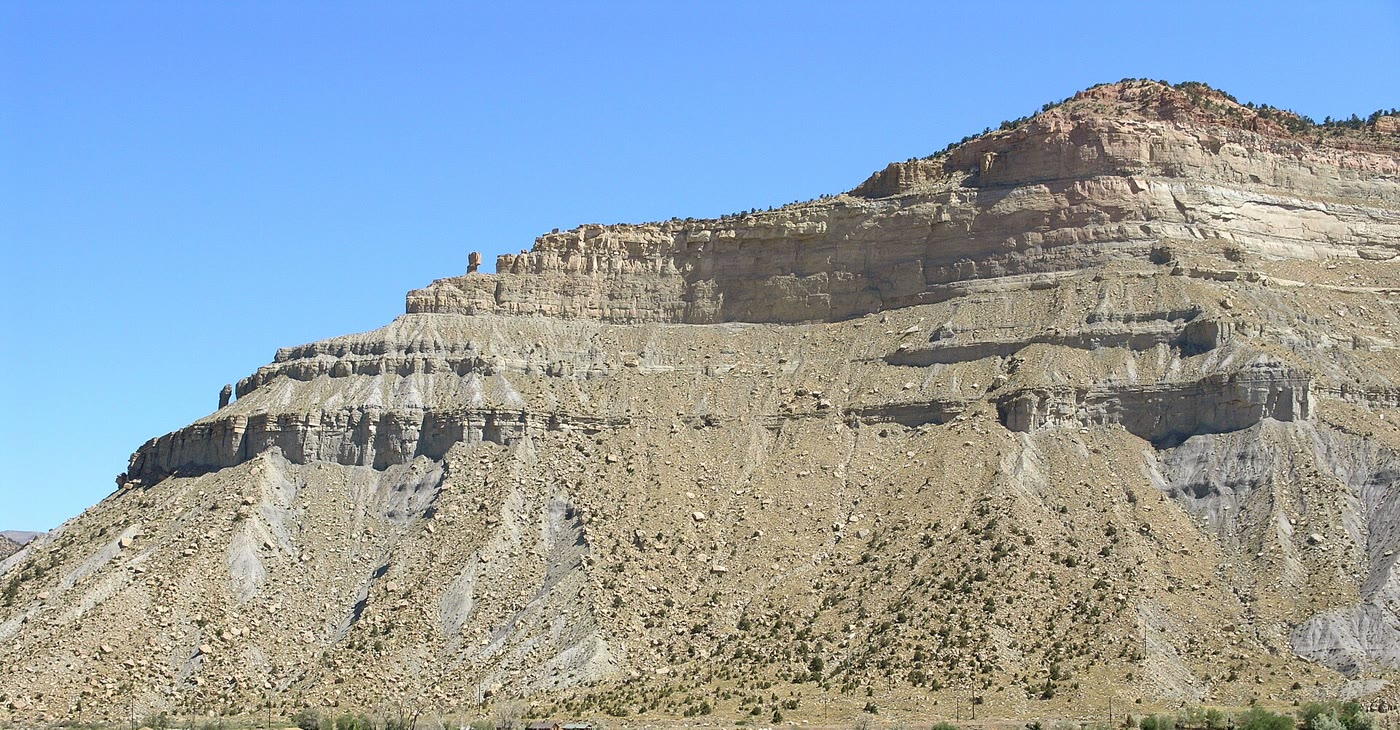
\includegraphics[width=\linewidth]{images/book5/b3-book-cliffs-helper.jpg}

{\scriptsize 犹他州海尔珀上方的布克悬崖：浅色砂岩陡壁突出于
灰色泥岩坡之上。照片：David Mackie，公有领域。}
\end{minipage}
\end{inthefield}
% ledger: pattison95:kenilworth, photo:b3-book-cliffs

\section{陆架正演模型}\label{sec:b3:sequence-stratigraphy:model}

前几节的规则可以用一个模型来运行。瓦尔登盆地是一个虚构的陆架：
一个向盆地方向倾斜、坡度为 \qty{1.5}{m/km} 的斜坡，
以 $\sigma = 0.02 + x/1200$ \unit{m/ka} 的速率沉降，$x$ 为距铰链点的距离（km），
海平面为 $E = -30\cos(2\pi t/400)$（m，$t$ 以 ka 计），
由一条河流供给沉积物，供给量为每米海岸 $Q = \qty{6000}{m^3/ka}$。
每隔五百年为一个时间步长，盆地沉降；随后沉积物
填满一个平坦的顶积层直至海平面，凡旧地表位于水下之处皆如此，
其前方并有坡度 0.012 的前积层，岸线位置使所增加的体积
等于供给量；裸露的陆地不接受沉积，为简便起见
也不予侵蚀。模型从低位开始，
位于恒定海平面下形成的第一套楔状体之后。

\begin{omfigure}
\begin{tikzpicture}
\begin{groupplot}[group style={group size=1 by 2, vertical sep=0.35cm, x descriptions at=edge bottom},
  omrecord, width=0.86\linewidth, xmin=0, xmax=600,
  xtick={0,100,200,300,400,500,600},
  tick label style={font=\scriptsize}, label style={font=\small}]
\nextgroupplot[height=0.2\linewidth, ylabel={$E$ (m)}, ymin=-35, ymax=35,
  ytick={-30,0,30}]
\addplot[omDef, thick, domain=0:600, samples=121] {-30*cos(deg(2*pi*x/400))};
\nextgroupplot[height=0.3\linewidth, xlabel={时间（ka）}, ylabel={岸线 $x_s$（km）},
  ymin=0, ymax=60, ytick={0,20,40,60},
  scatter/classes={1={mark=*, red!70!black}, 2={mark=*, orange!80!black},
    3={mark=*, green!50!black}, 4={mark=*, blue!70!black}}]
% computed in figdata/bachelor-3/shelf_model.py
\addplot[scatter, only marks, mark size=0.9pt, scatter src=explicit symbolic]
  table[x=t, y=xs, meta=tract] {figdata/out/bachelor-3-shelf_model-shore.dat};
\node[font=\scriptsize, orange!60!black] at (axis cs:12,56) {LST};
\node[font=\scriptsize, green!40!black] at (axis cs:70,40) {TST};
\node[font=\scriptsize, blue!60!black] at (axis cs:160,6) {HST};
\node[font=\scriptsize, red!60!black] at (axis cs:300,22) {FSST};
\node[font=\scriptsize, orange!60!black] at (axis cs:415,57) {LST};
\node[font=\scriptsize, green!40!black] at (axis cs:520,45) {TST};
\node[font=\scriptsize, blue!60!black] at (axis cs:580,12) {HST};
\end{groupplot}
\end{tikzpicture}

\par\smallskip{\small 上图为瓦尔登模型的全球海平面；
下图为岸线位置，按\omterm{def:b3:sequence-stratigraphy:tract}{体系域}着色（\omterm{def:b3:sequence-stratigraphy:tract}{低位体系域}
橙色，\omterm{def:b3:sequence-stratigraphy:tract}{海侵体系域}绿色，\omterm{def:b3:sequence-stratigraphy:tract}{高位体系域}蓝色，\omterm{def:b3:sequence-stratigraphy:tract}{下降期体系域}红色），
仅由模型输出划分：岸线处相对海平面下降时为下降期，
岸线后退时为海侵；岸线在海平面上升中前进时为低位或\omterm{def:b3:sequence-stratigraphy:tract}{高位
体系域}，位于一次下降或海侵之后
。}\label{fig:b3:sequence-stratigraphy:series}
\end{omfigure}

上图追踪岸线随时间的迁移，下图给出它留下的沉积。
除充填与沉降外，模型中未写入任何规则，\omterm{def:b3:sequence-stratigraphy:tract}{体系域}由此自然出现。
开始时的低位楔位于很远的
海域一侧；第一次海侵中，海平面上升使岸线向陆推进\qty{38}{km}，
高位前积层随海平面上升减缓而再次向海推进。
随后下降开始，岸线被推向盆地一侧\qty{33}{km}，
用时\qty{187}{ka}，留下薄的下阶式前积层和出露的陆架，
其后即\omterm{def:b3:sequence-stratigraphy:tract}{下降期体系域}。随后依次出现新的低位楔、第二次海侵
及新的\omterm{def:b3:sequence-stratigraphy:tract}{高位体系域}。模型中\omterm{def:b3:sequence-stratigraphy:regression}{强迫海退}的速度
与命题中的公式符合，误差在百分之几以内；在
海平面上升时，模型中的顶积层并不均匀加积，因为沉降
向盆地方向增大，该公式只能作为参考。

\begin{omfigure}
\begin{tikzpicture}
\begin{axis}[omsection, width=0.95\linewidth, height=0.42\linewidth,
  xmin=0, xmax=70, ymin=-150, ymax=40, clip=true,
  xlabel={向盆地距离（km）}, ylabel={当前高程（m）},
  xtick={0,10,20,30,40,50,60,70}, ytick={-150,-100,-50,0},
  tick label style={font=\scriptsize}, label style={font=\small}]
% computed in figdata/bachelor-3/shelf_model.py
\addplot[fill=black!10, draw=none] table[x=x, y=z0] {figdata/out/bachelor-3-shelf_model-surfaces.dat} -- (axis cs:120,-300) -- (axis cs:0,-300) -- cycle;
\addplot[fill=orange!45, draw=none] table[x=x, y=z] {figdata/out/bachelor-3-shelf_model-poly1.dat};
\addplot[fill=green!45!black!35, draw=none] table[x=x, y=z] {figdata/out/bachelor-3-shelf_model-poly2.dat};
\addplot[fill=blue!25, draw=none] table[x=x, y=z] {figdata/out/bachelor-3-shelf_model-poly3.dat};
\addplot[fill=red!30, draw=none] table[x=x, y=z] {figdata/out/bachelor-3-shelf_model-poly4.dat};
\addplot[fill=orange!45, draw=none] table[x=x, y=z] {figdata/out/bachelor-3-shelf_model-poly5.dat};
\addplot[fill=green!45!black!35, draw=none] table[x=x, y=z] {figdata/out/bachelor-3-shelf_model-poly6.dat};
\addplot[fill=blue!25, draw=none] table[x=x, y=z] {figdata/out/bachelor-3-shelf_model-poly7.dat};
\addplot[black!45, very thin] table[x=x, y=z40] {figdata/out/bachelor-3-shelf_model-surfaces.dat};
\addplot[black!45, very thin] table[x=x, y=z80] {figdata/out/bachelor-3-shelf_model-surfaces.dat};
\addplot[black!45, very thin] table[x=x, y=z120] {figdata/out/bachelor-3-shelf_model-surfaces.dat};
\addplot[black!45, very thin] table[x=x, y=z160] {figdata/out/bachelor-3-shelf_model-surfaces.dat};
\addplot[black!45, very thin] table[x=x, y=z240] {figdata/out/bachelor-3-shelf_model-surfaces.dat};
\addplot[black!45, very thin] table[x=x, y=z280] {figdata/out/bachelor-3-shelf_model-surfaces.dat};
\addplot[black!45, very thin] table[x=x, y=z320] {figdata/out/bachelor-3-shelf_model-surfaces.dat};
\addplot[black!45, very thin] table[x=x, y=z360] {figdata/out/bachelor-3-shelf_model-surfaces.dat};
\addplot[black!45, very thin] table[x=x, y=z440] {figdata/out/bachelor-3-shelf_model-surfaces.dat};
\addplot[black!45, very thin] table[x=x, y=z480] {figdata/out/bachelor-3-shelf_model-surfaces.dat};
\addplot[black!45, very thin] table[x=x, y=z520] {figdata/out/bachelor-3-shelf_model-surfaces.dat};
\addplot[black!45, very thin] table[x=x, y=z560] {figdata/out/bachelor-3-shelf_model-surfaces.dat};
\addplot[black, thin] table[x=x, y=z600] {figdata/out/bachelor-3-shelf_model-surfaces.dat};
\addplot[black, only marks, mark=*, mark size=0.5pt] table[x=xs, y=zfinal] {figdata/out/bachelor-3-shelf_model-shore.dat};
\node[font=\scriptsize, blue!50!black] at (axis cs:6,4) {HST};
\node[font=\scriptsize, green!30!black] at (axis cs:12,-22) {TST};
\node[font=\scriptsize, red!60!black] at (axis cs:35,-25) {FSST};
\node[font=\scriptsize, orange!60!black] at (axis cs:57.5,-60) {LST};
\node[font=\scriptsize, green!30!black] at (axis cs:36,2) {TST};
\node[font=\scriptsize, blue!50!black] at (axis cs:8,26) {HST};
\end{axis}
\end{tikzpicture}

\par\smallskip{\small 瓦尔登陆架在 \qty{600}{ka} 后，处于现今位置
（竖直方向放大约 170 倍）。颜色代表
\omterm{def:b3:sequence-stratigraphy:tract}{体系域}：低位为橙色，海侵为绿色，高位为蓝色，
下降期为红色；灰色为较老的斜坡及第一个楔体。细线为
每隔 \qty{40}{ka} 的海底面；黑点为每隔
\qty{2}{ka} 的岸线位置。由
文中的正演模型计算得出。}\label{fig:b3:sequence-stratigraphy:section}
\end{omfigure}


岸线处相对海平面在全球海平面高位之后数千年开始下降，
因为沉降须先被抵消，
并在全球海平面低位之前数千年结束。岸线处的
下降因此持续时间不足全球旋回的一半，盆地沉降越快，
则持续时间越短。

此类模型是检验解释是否可靠的有效手段，也能显示
其局限。同一剖面可由不同的历史形成：较快的下降加较少的供给，
或较慢的下降加较多的供给，或沉降变化而非海平面变化，
因为几何形态只记录相对海平面与供给
。根据 1970 年代和 1980 年代的陆缘资料建立的全球海平面旋回图表
确定了许多次下降的时间，此后钻探大体证实了这些时间，
适用于晚白垩世至中新世的部分时段，但其幅度，
幅度，例如中渐新世\qty{160}{m}的下降，
偏高 2 至 3 倍。目前全球海平面幅度取自
氧同位素与回剥井的资料，而陆缘的层序
首先应作为局地记录来解读。
% ledger: miller20:epr, miller20:rsl

\section{旋回地层学}\label{sec:b3:sequence-stratigraphy:cyclo}

许多地层序列以规则的厚度间隔重复：由泥灰岩与石灰岩组成的
韵律对、由五个韵律对组成的束，以及更大的束组。若
这种重复受米兰科维奇参数控制，则
旋回的厚度即可转换为时间。

\begin{definition}[旋回地层学与天文调谐]\label{def:b3:sequence-stratigraphy:cyclo}
\emph{旋回地层学}\index{旋回地层学}识别并测量\omterm{def:b3:sequence-stratigraphy:sequence}{沉积层序}中
的规则旋回，并将其解释为
周期性强迫的记录，主要是地球轨道与地轴的变化。
\emph{天文调谐}\index{天文调谐}为地层序列赋予年龄，方法是将其
旋回逐一与计算得到的天文序列（偏心率、斜交角、岁差
或日射量）相匹配，
从而将旋回转化为年龄模型。
\end{definition}

计算所得的周期来自太阳系运动方程的解。
地球轨道的偏心率主项为 \qty{405}{ka}，
另有四项接近 \qty{100}{ka}（95、99、124 和 \qty{131}{ka}）；
斜交角主项为 \qty{41.0}{ka}，较小的项位于 39.6 和
\qty{53.7}{ka}。气候岁差结合了地轴的岁差
与近日点的运动，频率为 $p_0 + g_i$，其中 $p_0 =
50.47''$ 每年，$g_i$ 为各行星轨道的频率；其
主要周期为 23.7、22.4、19.1 和 \qty{19.0}{ka}。\qty{405}{ka}
项最稳定，可作为较老地层序列的“节拍器”。
% ledger: la04:eccentricity, la04:obliquity, la04:precession

\begin{omfigure}
\begin{tikzpicture}
\begin{groupplot}[group style={group size=2 by 1, horizontal sep=0.5cm, y descriptions at=edge left},
  omrecord, width=0.52\linewidth, height=0.33\linewidth,
  xmin=0, xmax=0.06, ymin=0, ymax=1.18, clip=false,
  xtick={0,0.02,0.04,0.06}, xticklabels={0,0.02,0.04,0.06}, scaled x ticks=false,
  ytick={0,0.5,1}, title style={font=\small},
  tick label style={font=\scriptsize}, label style={font=\small},
  xlabel={频率（每千年周数）}]
\nextgroupplot[title={(a) 0 至 \qty{1000}{ka}}, ylabel={相对功率}]
\draw[black!40, densely dotted] (axis cs:0.01,0) -- (axis cs:0.01,1.05);
\draw[black!40, densely dotted] (axis cs:0.0244,0) -- (axis cs:0.0244,1.05);
\draw[black!40, densely dotted] (axis cs:0.0429,0) -- (axis cs:0.0429,1.05);
\draw[black!40, densely dotted] (axis cs:0.0526,0) -- (axis cs:0.0526,1.05);
\node[font=\scriptsize, anchor=south] at (axis cs:0.01,1.05) {100};
\node[font=\scriptsize, anchor=south] at (axis cs:0.0244,1.05) {41};
\node[font=\scriptsize, anchor=south] at (axis cs:0.0429,1.05) {23};
\node[font=\scriptsize, anchor=south] at (axis cs:0.0526,1.05) {19};
% computed in figdata/bachelor-3/lr04_periodogram.py
\addplot[omDef, thick] table[x=f, y=p] {figdata/out/bachelor-3-lr04_periodogram-young.dat};
\nextgroupplot[title={(b) 1250 至 \qty{2500}{ka}}]
\draw[black!40, densely dotted] (axis cs:0.01,0) -- (axis cs:0.01,1.05);
\draw[black!40, densely dotted] (axis cs:0.0244,0) -- (axis cs:0.0244,1.05);
\draw[black!40, densely dotted] (axis cs:0.0429,0) -- (axis cs:0.0429,1.05);
\draw[black!40, densely dotted] (axis cs:0.0526,0) -- (axis cs:0.0526,1.05);
\node[font=\scriptsize, anchor=south] at (axis cs:0.01,1.05) {100};
\node[font=\scriptsize, anchor=south] at (axis cs:0.0244,1.05) {41};
\node[font=\scriptsize, anchor=south] at (axis cs:0.0429,1.05) {23};
\node[font=\scriptsize, anchor=south] at (axis cs:0.0526,1.05) {19};
\addplot[omDef, thick] table[x=f, y=p] {figdata/out/bachelor-3-lr04_periodogram-old.dat};
\end{groupplot}
\end{tikzpicture}

\par\smallskip{\small 底栖氧同位素叠层 LR04 的\omterm{def:b3:sequence-stratigraphy:periodogram}{周期图}，
分两个时段（去趋势，Hann 锥度，按最大峰归一化）；
虚线标出周期为 100、41、23 和 \qty{19}{ka}。（a）最近
一百万年：\qty{100}{ka} 频带占主导。（b）自 2.5 至
\qty{1.25}{Ma}：\qty{41}{kyr} 的斜交角占主导。}\label{fig:b3:sequence-stratigraphy:periodogram}
\end{omfigure}
% ledger: data:lr04, lr04:tuning

\begin{definition}[周期图]\label{def:b3:sequence-stratigraphy:periodogram}
\emph{周期图}\index{周期图}是指序列 $y_0, \dots, y_{N-1}$
以步长 $\Delta$（时间或深度）采样，去除其均值与
趋势并乘以锥度 $w_k$ 后，为
\[
P(f_j) = \Bigl|\sum_{k=0}^{N-1} w_k y_k\, e^{-2\pi i f_j k\Delta}\Bigr|^2,
\qquad f_j = \frac{j}{N\Delta},\ j = 1, \dots, \frac N2:
\]
即序列在各频率 $f_j$ 处的功率，等于其离散
傅里叶变换的模的平方。
\end{definition}

\omterm{def:b3:sequence-stratigraphy:periodogram}{周期图}所能分辨的范围由两个数决定。其频率步长 $1/(N\Delta)$，
即记录长度的倒数，是分辨率：频率之差小于它的
两个周期无法分开。其最高频率为奈奎斯特频率 $1/(2\Delta)$，
每周期取两个样本即可达到；比它更短的
周期并不会丢失，而是被折叠为一个虚假的较长周期。锥度
（此处为 Hann 窗）平滑序列两端，使强峰
不会将功率泄漏到整个谱上。


上面的\omterm{def:b3:sequence-stratigraphy:periodogram}{周期图}即为示例。最近一百万年内，最强峰
位于 \qty{100}{ka} 频带（在 \qty{1000}{ka} 记录的
频率网格上位于 \qty{91}{ka}，其相邻值为 100 和 \qty{83}{ka}），
斜交角的功率约为其三分之一，岁差的功率仅为百分之几；
在 2.5 至 \qty{1.25}{Ma} 之间，斜交角承载了整个记录，而
\qty{100}{ka} 频带的功率仅为其六分之一。数据中内含一项需要留意之处：
LR04 时间标尺本身是通过将叠层调谐至一个简单的
冰模型得到的，此冰模型由北纬 \ang{65} 的夏季日射量驱动，并以叠加的
沉积速率加以约束，以防过度调谐，因此在其中寻找轨道周期
在一定程度上是循环论证的。不循环的检验
是在任何调谐之前、在深度上进行的：若旋回厚度之比与
轨道周期之比相符，则证明了强迫作用，厚度即可给出
沉积速率。
% ledger: lr04:tuning, la04:obliquity

\begin{method}[由旋回厚度求沉积速率]\label{met:b3:sequence-stratigraphy:cycles}
\begin{enumerate}
\item 对深度序列计算\omterm{def:b3:sequence-stratigraphy:periodogram}{周期图}，其分辨率为
  $1/L$（$L$ 为剖面长度），奈奎斯特极限为 $1/(2\Delta z)$；
\item 列出显著峰的波长 $\lambda = 1/f$；
\item 将其比值与轨道周期之比（405 : 100 : 41
  : 23，平均岁差取 21）相比较；三个峰相符是有力的
  论据，仅一个峰则不足为凭；
\item 将每个波长除以其周期：所得商应当
  相等，即为沉积速率。
\end{enumerate}
\end{method}

以此方法得到的沉积速率是旋回上的平均值，并
假定速率恒定：剖面内速率的变化会拉伸
峰形，而间断会无声地去除旋回。因此，长序列
需逐旋回对照计算序列进行调谐，先调谐 \qty{405}{ka} 旋回，
并在火山岩层允许处与放射性年龄相核对。

\section{练习}

\begin{exercise}[$\star$]\label{exo:b3:sequence-stratigraphy:1}
在陆架上某一点，全球海平面以 \qty{0.5}{m/ka} 上升，
盆地以 \qty{0.1}{m/ka} 沉降。求相对
海平面上升速率，以及在 \qty{20}{ka} 内形成的可容纳空间。
若海平面改以 \qty{0.3}{m/ka} 下降，相对速率为多少？
\end{exercise}

\begin{exercise}[$\star$]\label{exo:b3:sequence-stratigraphy:2}
对下列各情形，指出正在形成的\omterm{def:b3:sequence-stratigraphy:tract}{体系域}：（a）相对海平面
下降，岸线向海推进；（b）相对海平面上升，
岸线向陆迁移；（c）旋回后期相对海平面缓慢上升，
岸线向海推进，且前积层\omterm{def:b3:exploration-seismology:terminations}{下超}于
\omterm{def:b3:sequence-stratigraphy:surfaces}{最大海泛面}之上；（d）相对海平面刚由下降转为上升，
岸线仍向海推进。
\end{exercise}

\begin{exercise}[$\star$]\label{exo:b3:sequence-stratigraphy:3}
一条测井曲线显示三个\omterm{def:b3:sequence-stratigraphy:parasequence}{准层序}，每个都向上变粗。
自下而上，三者顶部分别为细砂、中砂和带滩面层理的粗砂。
说明其叠加样式、岸线的迁移方向，
以及它们可能所属的\omterm{def:b3:sequence-stratigraphy:tract}{体系域}。若顺序相反，又意味着什么？
\end{exercise}

\begin{exercise}[$\star$]\label{exo:b3:sequence-stratigraphy:4}
一处悬崖露出泥灰岩与石灰岩的互层，每五个互层组成一束，
每束厚 \qty{1.6}{m}。试用轨道周期解释互层与束状结构，
并由束的厚度计算沉积速率。
\end{exercise}

\begin{exercise}[$\star\star$]\label{exo:b3:sequence-stratigraphy:5}
某陆架的顶积层宽 \qty{20}{km}，前积层高 \qty{50}{m}，
每米海岸的供给量为 \qty{4000}{m^3/ka}；相对海平面以
\qty{0.15}{m/ka} 上升。求岸线的速度。以多大的上升速率，
岸线会保持静止？
\end{exercise}

\begin{exercise}[$\star\star$]\label{exo:b3:sequence-stratigraphy:6}
同一陆架上，相对海平面现以 \qty{0.2}{m/ka} 下降；
前积层坡度为 0.01。求\omterm{def:b3:sequence-stratigraphy:regression}{强迫海退}的速度，以及
其中仅由海平面下降引起的部分。
\end{exercise}

\begin{exercise}[$\star\star$]\label{exo:b3:sequence-stratigraphy:7}
相对海平面以 \qty{0.4}{m/ka} 上升，顶积层宽 \qty{25}{km}。
供给量低于多少时岸线会后退？若每米供给量为
\qty{6000}{m^3/ka}，而临滨高仅 \qty{10}{m}，
岸线后退的速度为多少？
\end{exercise}

\begin{exercise}[$\star\star$]\label{exo:b3:sequence-stratigraphy:8}
偏心率项的周期分别为 94.9 与 \qty{123.9}{ka}，以及 94.9 与
\qty{98.9}{ka}：在\omterm{def:b3:sequence-stratigraphy:periodogram}{周期图}中区分每一对至少需要多长的记录？
长度为 \qty{600}{ka} 的记录能否做到？
\end{exercise}
% ledger: la04:eccentricity

\begin{exercise}[$\star\star$]\label{exo:b3:sequence-stratigraphy:9}
某岩芯中，20 个斜率周期（每个 \qty{40.98}{ka}）占据
\qty{16.4}{m}。求沉积速率，以及同一层段中
相距 \qty{3.1}{m} 的两层火山灰之间的时间间隔。
\end{exercise}
% ledger: la04:obliquity

\begin{exercise}[$\star\star\star$]\label{exo:b3:sequence-stratigraphy:10}
求\omterm{def:b3:sequence-stratigraphy:trajectory}{岸线轨迹}的角度：（a）\omterm{def:b3:sequence-stratigraphy:regression}{强迫海退}中，岸线速度为
\qty{200}{m/ka}，相对海平面以 \qty{0.4}{m/ka} 下降；（b）\omterm{def:b3:sequence-stratigraphy:regression}{正常海退}中，
岸线速度为 \qty{50}{m/ka}，相对海平面以
\qty{0.2}{m/ka} 上升。为什么不足一度的角度在地震剖面上容易看出，
在悬崖上却难以辨认？
\end{exercise}

\begin{exercise}[$\star\star\star$]\label{exo:b3:sequence-stratigraphy:11}
岁差常数为 $p_0 = 50.467718''$ 每年，四个行星频率分别为
$g_5 = 4.257564$、$g_2 = 7.456665$、$g_4 = 17.910194$ 和
$g_3 = 17.366595''$ 每年。计算气候岁差的周期
$1\,296\,000''/(p_0 + g_i)$。验证 $g_2 - g_5$ 与 $g_4 - g_5$ 给出
405 与 \qty{95}{ka} 的偏心率项。
\end{exercise}
% ledger: la04:precession, la04:eccentricity

\begin{exercise}[$\star\star\star$]\label{exo:b3:sequence-stratigraphy:12}
两个盆地记录了相同的相对海平面上升，速率为 \qty{0.3}{m/ka}，持续
\qty{100}{ka}。第一个盆地中，全球海平面以 \qty{0.25}{m/ka} 上升，
盆地以 \qty{0.05}{m/ka} 沉降；第二个盆地中，全球海平面以
\qty{0.1}{m/ka} 上升，盆地以 \qty{0.2}{m/ka} 沉降。证明这两个
剖面可以完全相同。还需要什么额外的观察，才能区分这两段
历史？
\end{exercise}

\section{问题：瓦尔登盆地的海平面}

\begin{problem}[{周末问题——可容纳空间、瓦尔登陆架模型的岸线轨迹与
体系域，以及岩芯的时钟}]
\label{pb:b3:sequence-stratigraphy:1}
本章的瓦尔登陆架以 $\sigma = 0.02 + x/1200$
（\unit{m/ka}，$x$ 以 km 计）沉降，海平面为 $E = -30\cos(2\pi t/400)$（m，
$t$ 以 ka 计），每米海岸的供给量为 \qty{6000}{m^3/ka}，以及
前积层坡度为 0.012。模型每隔 \qty{50}{ka} 给出海平面
$E$、岸线位置 $x_s$、岸线处相对海平面上升速率
$A$ 以及前积层高度 $D$：

\begin{center}\small
\begin{tabular}{rrrrr|rrrrr}
$t$ & $E$ & $x_s$ & $A$ & $D$ & $t$ & $E$ & $x_s$ & $A$ & $D$\\
(ka) & (m) & (km) & (m/ka) & (m) & (ka) & (m) & (km) & (m/ka) & (m)\\\hline
50 & $-21.2$ & 33.5 & 0.381 & -- & 350 & $-21.2$ & 44.6 & $-0.276$ & 25.3\\
100 & 0.0 & 15.7 & 0.504 & -- & 400 & $-30.0$ & 51.3 & 0.063 & 81.6\\
150 & 21.2 & 12.8 & 0.364 & 21.1 & 450 & $-21.2$ & 52.7 & 0.397 & 99.2\\
200 & 30.0 & 16.8 & 0.034 & 41.1 & 500 & 0.0 & 40.4 & 0.525 & --\\
250 & 21.2 & 24.0 & $-0.293$ & 45.4 & 550 & 21.2 & 22.9 & 0.372 & --\\
300 & 0.0 & 32.9 & $-0.424$ & 35.7 & 600 & 30.0 & 28.2 & 0.043 & 13.4\\
\end{tabular}
\end{center}
（“--”表示岸线在平坦的海岸平原上后退，
此处不形成前积层。）

\medskip\noindent\textbf{第一部分——可容纳空间。}
\begin{enumerate}
\item 计算最大的全球海平面变化速率，以及它出现的时刻。
\item 计算转折端的沉降速率，分别在 20 与 \qty{50}{km} 处，以及
  模型边缘 \qty{120}{km} 处的沉降速率。
\item 高位期岸线位于 \qty{17.5}{km} 附近。相对海平面何时
  开始在该处下降？
\item 低位期岸线到达约 \qty{50}{km}。相对海平面何时
  停止在该处下降？
\item 岸线处相对海平面的下降持续多久，与
  \qty{200}{ka} 的全球海平面下降相比如何？为什么更短？
\item 仅由沉降在一个旋回内于
  \qty{30}{km} 处产生多少可容纳空间？与全球海平面的变化幅度相比如何？
\end{enumerate}

\medskip\noindent\textbf{第二部分——岸线。}
\begin{enumerate}[resume]
\item 阅读下表：岸线在哪些时段向海推进，
  以及哪些时段向陆后退？
\item 一个高位顶积层宽 \qty{15}{km}，以 \qty{0.30}{m/ka} 的速率加积，
  位于高 \qty{40}{m} 的前积层前方。利用本章的命题计算
  岸线的速度。
\item 在该顶积层上，抬升速率为多少时岸线会停止移动？
\item 在 \qty{300}{ka} 时，计算\omterm{def:b3:sequence-stratigraphy:regression}{强迫海退}的速度，
  依据表格。模型给出 \qty{204}{m/ka}：请比较二者。
\item 两项中哪一项占主导，是供给还是下降？
\item 轨迹由 \qty{17.4}{km}（\qty{204.5}{ka}）处的 \qty{16.3}{m}
  下降至 \qty{50.7}{km}（\qty{391.5}{ka}）处的 \qty{-42.7}{m}，
  均为现今高程。计算其平均梯度。
  由每一点此后经历的沉降，说明这一下降为何
  几乎等于 \qty{59.7}{m} 的全球海平面下降。
\end{enumerate}

\medskip\noindent\textbf{第三部分——层序\omterm{def:b3:sequence-stratigraphy:tract}{体系域}。}
\begin{enumerate}[resume]
\item 根据表格，为 150 至
  \qty{600}{ka} 之间的每个时刻指定一个层序\omterm{def:b3:sequence-stratigraphy:tract}{体系域}。
\item 模型给出下降期的开始时刻为 \qty{204.5}{ka}，
  结束时刻为 \qty{391.5}{ka}：请对照第 3 题和第 4 题进行检验。
\item 在该模型中，\omterm{def:b3:sequence-stratigraphy:sequence}{层序界面}在陆架上和
  盆地中各形成于何处？模型不含侵蚀：真实的陆架会呈现怎样的情形？
\item 第二次海侵于 \qty{559}{ka} 结束，此时岸线位于
  \qty{18.5}{km} 处。计算其平均速度，起点位于 \qty{52.8}{km} 处，
  时刻为 \qty{439.5}{ka}。其结束时形成哪一种界面？
\item 为什么\omterm{def:b3:sequence-stratigraphy:tract}{海侵体系域}在陆架上很薄，
  \omterm{def:b3:sequence-stratigraphy:condensed}{凝缩段}又会形成于何处？
\end{enumerate}

\medskip\noindent\textbf{第四部分——盆地中的一根岩芯。}岩芯
长 \qty{30}{m}，每厘米取样一次，显示出规则的交替变化；其
按深度计算的\omterm{def:b3:sequence-stratigraphy:periodogram}{周期图}在波长为 7.5、2.0 和 \qty{0.81}{m} 处有峰值，
其中最大峰位于 \qty{2.0}{m} 处。
\begin{enumerate}[resume]
\item 计算该\omterm{def:b3:sequence-stratigraphy:periodogram}{周期图}的频率分辨率和
  奈奎斯特频率。
\item 计算三个波长与最大峰的比值，并
  将其与轨道周期进行比较。
\item 为各峰指定周期，并由每个峰
  计算沉积速率。为什么最长的那个峰与其他结果略有不符？
\item 这根岩芯覆盖了多长时间？
\item 岁差（周期 \qty{23.7}{ka}）应在何种波长处出现？
  若岩芯每 \qty{25}{cm} 取样一次，能否观测到它，它又落在何处？
\item 为什么三个峰的吻合比单个峰更有说服力？
\item 指出模型中岸线向盆地方向的最大位移，
  自下降开始至低位海退结束。
\end{enumerate}
\end{problem}
% ledger: la04:eccentricity, la04:obliquity, la04:precession
